%% §4 — Performance  (4 slides)
\section{Performance \& Comparison}

%% ── Slide 14: Memory scaling ────────────────────────────────────────────────
\begin{frame}{Memory Scaling: Dense vs.\ H-Matrix}
\begin{columns}[T]
\begin{column}{0.50\textwidth}
  \centering
  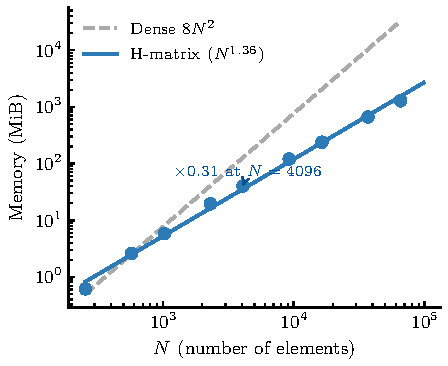
\includegraphics[width=0.96\linewidth]{figures/fig_memory_scaling.pdf}
\end{column}
\begin{column}{0.46\textwidth}
  \begin{block}{Key numbers at $N=4096$ ($N_s=64$)}
    \begin{tabular}{lc}
      \toprule
      Quantity & Value \\
      \midrule
      Dense storage & 128\,MiB \\
      H-matrix storage & 40\,MiB \\
      \textbf{Compression} & \textbf{0.31$\times$} \\
      Dense blocks & 2\,116 \\
      Low-rank blocks & 6\,900 \\
      Avg.\ rank $k$ & 11 \\
      \bottomrule
    \end{tabular}
  \end{block}
  \vspace{0.3em}
  At $N_s=256$ ($N=65\,536$):\\
  H-matrix: 1.3\,GB \quad vs.\quad
  Dense: \alert{34\,GB}
  \vspace{0.2em}

  Fit exponent $\approx N^{1.45}$ in practice
  (target $O(N\log^2 N) \approx N^{1.28}$ at $N\!=\!4096$)
\end{column}
\end{columns}
\end{frame}

%% ── Slide 15: Timing scaling ────────────────────────────────────────────────
\begin{frame}{Timing Scaling: Assembly \& Matvec vs.\ $N$}
\begin{columns}[T]
\begin{column}{0.50\textwidth}
  \centering
  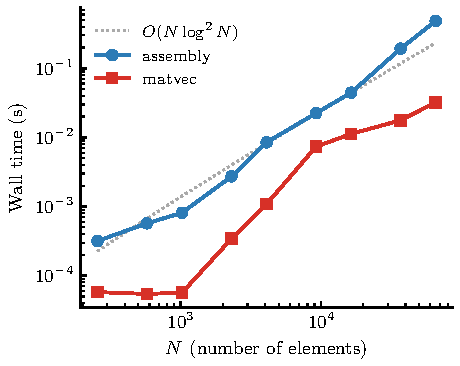
\includegraphics[width=0.96\linewidth]{figures/fig_timing_scaling.pdf}
\end{column}
\begin{column}{0.46\textwidth}
  \begin{block}{Measured wall times (20-core Xeon)}
    \centering
    \begin{tabular}{rrr}
      \toprule
      $N_s$ & Assembly & Matvec \\
      \midrule
       64 &   7\,ms  &  0.6\,ms \\
      128 &  44\,ms  &  11\,ms \\
      256 & 484\,ms  &  32\,ms \\
      \bottomrule
    \end{tabular}
  \end{block}
  \vspace{0.4em}
  \begin{itemize}
    \item Assembly parallelised with OpenMP
    \item Matvec: 9\,016 block GEMVs
      (independent $\to$ OpenMP)
    \item Both roughly $O(N\log^2 N)$
    \item Matvec dominated by low-rank
      blocks ($k\approx11$)
  \end{itemize}
\end{column}
\end{columns}
\end{frame}

%% ── Slide 16: Comparison with Tamaas ────────────────────────────────────────
\begin{frame}{Comparison with Tamaas (Non-Periodic)}
\begin{columns}[T]
\begin{column}{0.52\textwidth}
  \centering
  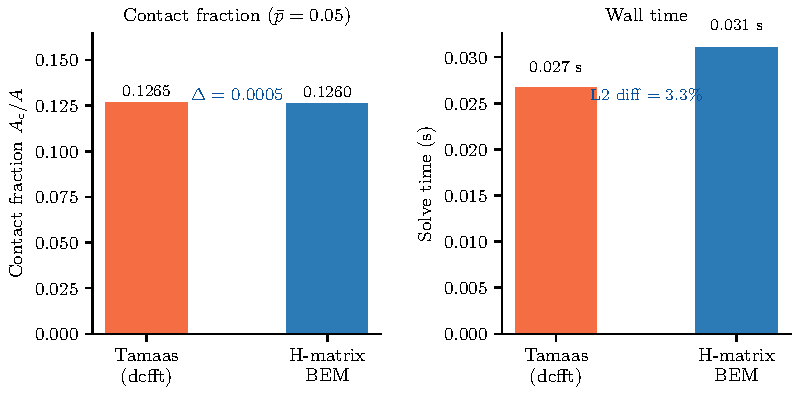
\includegraphics[width=0.96\linewidth]{figures/fig_tamaas_comparison.pdf}
\end{column}
\begin{column}{0.44\textwidth}
  \begin{block}{Summary ($N_s=64$, $\pbar=0.05$)}
    \begin{tabular}{lcc}
      \toprule
      Metric & Tamaas & BEM \\
      \midrule
      $A_c/A$ & 0.1265 & 0.1260 \\
      $|\Delta A_c/A|$ & \multicolumn{2}{c}{0.0005} \\
      $\langle p\rangle / \pbar - 1$ & $<10^{-14}$ & $<10^{-14}$ \\
      Iters & 33 & 26 \\
      $\|p_\mathrm{BEM}-p_\mathrm{T}\|/\|p_\mathrm{T}\|$ &
        \multicolumn{2}{c}{3.3\,\%} \\
      \bottomrule
    \end{tabular}
  \end{block}
  \vspace{0.3em}
  \small
  The 3.3\,\% L2 difference is dominated by\\
  Gibbs-like near-field errors in Tamaas\\
  dcfft operator ($\pm2$--$8$\,\% at $r=1$--$3h$),\\
  \emph{not} by the H-matrix approximation.
\end{column}
\end{columns}
\end{frame}

%% ── Slide 17: Conclusions ───────────────────────────────────────────────────
\begin{frame}{Conclusions}
\begin{columns}[T]
\begin{column}{0.55\textwidth}
  \textbf{Delivered}:
  \begin{itemize}
    \item C++17 H-matrix BEM library
      (\texttt{libhmatrix\_contact + Python module})
    \item Love element kernel (exact, $O(1)$ lookup)
    \item Quad-tree + ACA ($\varepsilon_{\rm aca}=10^{-6}$)
    \item Polonsky--Keer PCG solver
    \item OpenMP-parallel assembly \& matvec
  \end{itemize}

  \vspace{0.5em}
  \textbf{Validated}:
  \begin{itemize}
    \item Hertz: $a_{\rm num}/a = 1.016$,
      $p_{\rm max}/p_0 = 0.998$
    \item H-matvec vs.\ dense: $<10^{-5}$ rel.\ L2
    \item Rough contact vs.\ Tamaas: $|\Delta A_c|=0.0005$
  \end{itemize}
\end{column}
\begin{column}{0.40\textwidth}
  \begin{block}{Outlook}
    \begin{itemize}
      \item Larger grids via MPI\\
        ($N_s \sim 10^3$, $N\sim10^6$)
      \item Plasticity (Mindlin--Deresiewicz)
      \item Adhesion (JKR / DMT)
      \item 3D bodies (volume BIE)
      \item Non-conforming surface meshes
    \end{itemize}
  \end{block}
  \vspace{0.4em}
  \small
  Code: \texttt{Hcontact/} \\
  Build:
  \begin{itemize}
    \item \texttt{cmake -S . -B build}\\
      \texttt{\;\;-DCMAKE\_CXX\_COMPILER=/usr/bin/g++}
    \item \texttt{cmake --build build -j}
    \item \texttt{ctest --test-dir build}
  \end{itemize}
\end{column}
\end{columns}
\end{frame}
